\chapter[Resultados Alcançados]{Resultados Alcançados}

O primeiro objetivo alcançado foi a apresentação da fundamentação teórica sobre $Behavior$ $Driven$ $Development$ (BDD), contido na introdução deste relatório. Outro objetivo alcançado foi a apresentação da ferramenta de testes Letucce juntamente com o plugin zope.testbrowser, que foram utilizados no desenvolvimento dos testes neste projeto, juntamente com um pequeno tutorial de instalação, configuração junto ao Django e desenvolvimento de uma funcionalidade básica.

Outro objetivo alcançdo, foi a apresentação de testes implementados utilizando a ferramenta Letucce no software em desenvolvimento Busine.me, que foi escolhido para receber os testes no decorrer do projeto. Estes testes já implementados, descrevem dois usos diferentes de a ferramenta Letucce, um com o plugin zope.testbrowser e outro sem, para mostrar duas formas diferentes de se imlpementar os testes com a ferramenta designada. 

Um objetivo parcialmente alcançado neste ponto do projeto é o guia de implementação BDD em português para Python/Django usando a ferramenta Lettuce, focando contribuir na consolidação de fontes de informações de uso. Este guia está parcialmente concluído pois um de seus componentes, que é o tutorial de instalação e configuração da ferramenta Letucce e um pequeno roteiro de implementação dos testes, foi um dos objetivos já alcançados no projeto.

O produto a ser desenvolvido é relevante pois os testes utilizando $Behavior$ $Driven$ $Development$ (BDD) ainda não são bem implementados pois possuem poucas referências de como se fazer ou do uso e descrição de ferramentas que podem auxiliar na produção destes tipos de testes.

Para o relatório final deverão ser cumpridos os objetivos de desenvolvimento do guia de implementação BDD para Python/Django e o suporte de implementação com o tutorial em vídeo do desenvolvimento dos testes. Sendo que assim que alcançados estes objetivos os resultados alcançados do projeto estarão completos.

Para o desenvolvimento desse relatório foi seguido o cronograma representado na figura \ref{fig:cronograma} com algumas adaptações.

\begin{figure}[h!]
        \centering
        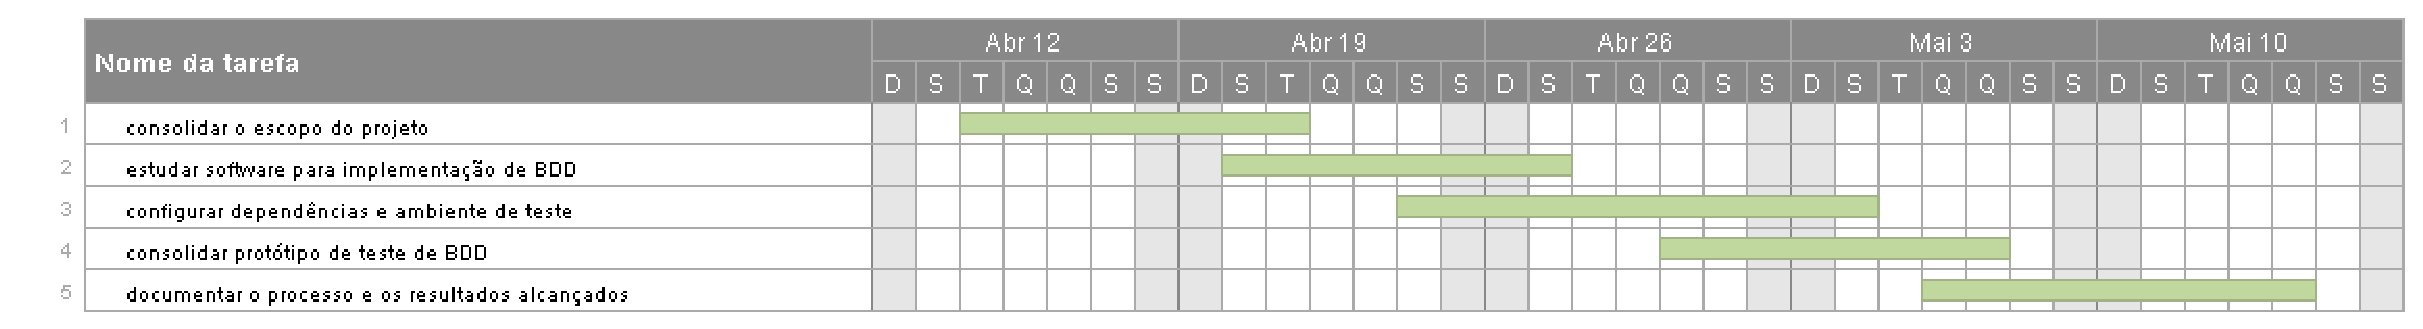
\includegraphics[width=1.1\textwidth]{figuras/verival.eps}
        \caption{Cronograma para a Segunda Entrega}
        \label{fig:cronograma}
\end{figure}
